\documentclass[12pt,tikz,border=10pt]{standalone}

\usepackage{pgfplots}
\usetikzlibrary{fillbetween}

%function={normal(\m,\s)=(1/(\s*sqrt(2*pi)))*exp(-(x-\m)^2/(2*\s^2));}

\begin{document}
	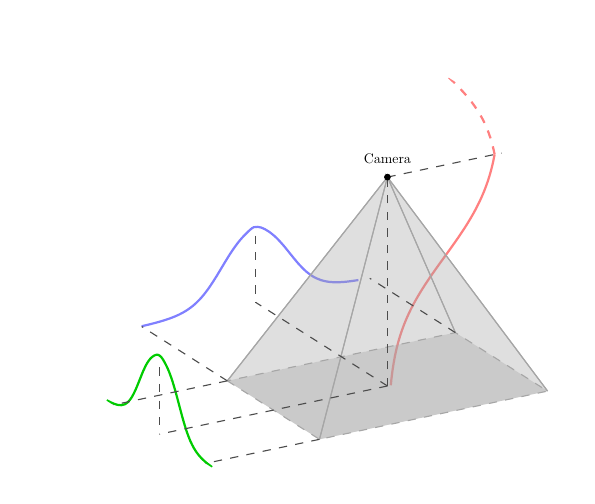
\begin{tikzpicture}[declare function={logic(\k,\f,\zz)= 1-(1/(1+exp(-\k*(abs(x-\zz)-\f)))));}
		]

		\begin{axis}[
			view={60}{30},
			samples=30,
			zmin= 0, zmax=3,
			xmin= 0, xmax=3,
			ymin= 0, ymax=3,
			ticks=none,
			axis line style={draw=none},
			]
			
			\addplot3 [ samples y=0,
				style={
				fill opacity=0.5,
				%draw=none,
				%fill=blue!50,
				color=blue!50,
				thick,
				mark=none,
				smooth,
				domain=1:2.9,
			}](0, x, {logic(8,0.3,2)});
	
			\addplot3 [samples y=0,
				style={
				%fill opacity=0.5,
				%draw=none,
				%fill=green!80!black,
				color=green!80!black,
				thick,
				mark=none,
				smooth,
				domain=1.2:2.8,
			}](x, 0, {logic(10,0.3,2)});
		
			\addplot3 [samples y=0,
				style={
				%fill opacity=0.5,
				%draw=none,
				color=red!50,
				%fill=red!90,
				mark=none,
				smooth,
				domain=0:2.5,
				thick,
			}](2, {2+logic(2.5,1.1,2.5)}, x);
		
			\addplot3 [samples y=0,
			style={
				%fill opacity=0.5,
				%draw=none,
				color=red!50,
				%fill=red!90,
				mark=none,
				smooth,
				domain=2.5:4,
				dashed,
				thick,
			}](2, {2+logic(2.5,1.1,2.5)}, x);
		
			\addplot3 [style={
				draw=gray!70,
				fill opacity=0.5,
				fill=gray!70,
				mark=none,
				dashed,
			}]coordinates {(1.3,1,0) (2.7,1,0) (2.7,3,0) (1.3,3,0) (1.3,1,0)};
		
			\addplot3 [style={
				draw=gray!70,
				fill opacity=0.2,
				fill=gray!70,
				mark=none,
			}]coordinates {(1.3,1,0) (2,2,2.5) (2.7,1,0)};	
		
			\addplot3 [style={
				draw=gray!70,
				fill opacity=0.2,
				fill=gray!70,
				mark=none,
			}]coordinates {(2.7,1,0) (2,2,2.5) (2.7,3,0)};	
		
			\addplot3 [style={
				draw=gray!70,
				fill opacity=0.2,
				fill=gray!70,
				mark=none,
			}]coordinates {(2.7,3,0) (2,2,2.5) (1.3,3,0)};	
		
			\addplot3 [style={
				draw=gray!70,
				fill opacity=0.2,
				fill=gray!70,
				mark=none,
			}]coordinates {(1.3,3,0) (2,2,2.5) (1.3,1,0)};
		
			\addplot3 [style={
				draw=black!70,
				dashed,
				mark=none
			}]coordinates {(2,2,0) (2,2,2.5)};
			
			\addplot3 [style={
				draw=black!70,
				dashed,
				mark=none
			}]coordinates {(2,2,0) (2,0,0)};
		
			\addplot3 [style={
				draw=black!70,
				dashed,
				mark=none
			}]coordinates {(2,0,0.8) (2,0,0)};
		
			\addplot3 [style={
				draw=black!70,
				dashed,
				mark=none
			}]coordinates {(2,2,0) (0,2,0)};
		
			\addplot3 [style={
				draw=black!70,
				dashed,
				mark=none
			}]coordinates {(0,2,0.8) (0,2,0)};
		
			\addplot3 [style={
				draw=black!70,
				dashed,
				mark=none
			}]coordinates {(2,2,2.5) (2,3,2.5)};
		
			\addplot3 [style={
				draw=black!70,
				dashed,
				mark=none
			}]coordinates {(1.3,1,0) (1.3,0,0)};
		
			\addplot3 [style={
				draw=black!70,
				dashed,
				mark=none
			}]coordinates {(2.7,1,0) (2.7,0,0)};
		
			\addplot3 [style={
				draw=black!70,
				dashed,
				mark=none
			}]coordinates {(1.3,3,0) (0,3,0)};
		
			\addplot3 [style={
				draw=black!70,
				dashed,
				mark=none
			}]coordinates {(1.3,1,0) (0,1,0)};
		
			\addplot3 [style={
				color=black,
				mark=*,
				mark size = 1pt,
			}]coordinates {(2,2,2.5)};
		
			\node[above, scale=0.5] at (axis cs: 2,2,2.6) {Camera};
		
		\end{axis}
	\end{tikzpicture}
\end{document}